\chapter{Techniques}
\label{Chapter4}
\lhead{Chapter 4. \emph{Codes}}

Throughout this thesis my goals were to identify SLSNe in a number of surveys. I have approached this problem using a variaty of tools and techniques which I describe in this chapter. The methods of classification SLSN described in this chapter span a number of methods. In the early parts of this thesis I used an approached based on modelling of SLSNe using the popular spin-down of a magnetar model \sref{sec:SLAP}. While this technique was successful in identifying a new SLSN in the SNLS it was found to be insufficient in the case of mode diverse but also noisy DES data. To solve this problem I have followed a popular path for classification style problems by approaching it using a machine learning approach. It is the preparation for the sample building methods, described further in \cref{Chapter5}, that form the second part of this chapter. The use of machine learning means that the majority of the work is not put into the understanding of the parameter space of the model applied to the data and any potential cuts that need to be made by currating and cleaning the data. Our approach is to simulate DES using all tranient models that are currently availabe to us. This includes similating SNIa, CCSN, SLSN as well as random noise and AGN activity.

While the models of SNIa are mature and ready to be applied to our work the simulations of CCSN could not have been accieved that easily. CCSN are usually faster and fainter than SNIa resulting is a significantly smaller sample of well observed objects. Most of them are also not observed using the same spectoscopic thoroughness making the a less understood class of objects. In recent years the interest in modeling this objects has increased dramatically with projects such as LSST underway. In this chapter I describe our approach to producing templates of CCSN as well as simulating them in a number of surveys. This project has originally been started as part of the LSST transients classification challenge however later I have applied it to DES to produce samples of both hydrogen rich and poor CCSN.

The last, but perhaps the most key, technique descrined in this chapter is Gaussian Processing. As the DES data was not observed on regular cadance, it would be impossible to apply any machine learning technique to good success to the row data. We used GPs as a method of modelling the confidence regions of the underlying light curves for the observed and simulated DES objects in a model-independant way. This was key as at the next stage of the process it would be "BAD" if instead of classifing the objects we uncover the underlying model instead of the data itself.

This chapter is divided in the following way. I begin by describing the method of modelling of SLSNe using the magnetar model in conjunction with SED templates. I then follow this by a discussion of the method as applied to the search for SLSNe in DES as well as their pre-peak 'bumps' and other rapidly evolving transients. Next, I describe the process of Gaussian Processing light curves as a model-independant approach to approximating the original data. Finally I describe the technique behind simulating samples of CCSN as used for machine learning classification of SLSNe.

\section{Modeling SLSN Light Curves} \label{sec:SLAP}
Throughout this thesis the modelling of SLSNe light curves plays a pivotal role. The measurement of the rate of SLSNe presented in \cref{Chapter3} as well as the search for SLSNe in DES described in \cref{Chapter5,Chapter6} uses a definition of SLSNe based on the spin-down of the magnetar model (magnetar model) [CITE]. In both cases a simpler model describing SLSNe using and linearly expanding and cooling photosphere has also been investigated but eventually rejected in favour of the magnetar model. I begin by giving a short decription of this model and its drawbacks before describing the improvements brought upon by the magnetar model. When modelling a SLSNe light curve there are two independant (but equally important) areas that contribute to the accuracy of the model: the spectral energy distribution (SED) of the SN, and its evolution with time.

The need to model the SED of a SN could be avoided if we used an approach which purely relied on the bolometric lightcurves as opposed to multi-band observations. While from the implemetation point of view these models are easier to use, and are common in the literature [CITE: Cosimo, Andreas and Nicolls], they do not take into consideration colour information about the SN which could provide further constraints for the properties of the SNe. It has been previously shown \citep{2011ApJ...743..114C,2013ApJ...779...98H,2015MNRAS.449.1215P,2014ApJ...797...24V} that the SLSN SED can be accurately approximated, in the visible spectrum, by a slowly evolving (nearly) perfect blackbody, with characteristic broad lines of \ion{O}{ii}. However, this approximation breaks down in the near UV due to the prominant broad absorption features which can be attributed to \ion{Mg}{ii}, \ion{Fe}{iii}, \ion{C}{ii}, \ion{Co}{iii}, \ion{Si }{iii} and \ion{Ti}{iii} \citep[see][for line identifications]{2016MNRAS.458.3455M}.

\subsection{Improving the blackbody approximation}
I propose a method of improving the blackbody approximation for the SLSN SED by superimposing absorption template onto the simple blackbody SED. In order to derive such template, I follow the method used in \citet{2014ApJ...797...24V} by fitting the Planck function to several featureless, 50$\AA$ wide regions of the spectrum in order to measure the underlined blackbody continuum in the SED, as shown in figure \ref{fig:specTemplate}. The resulting fits show that the absorption, relative to the blackbody, is low in the regions of $\lambda>3000\AA$, and increases drastically in the bluer regions of the spectrum.

The time evolution of the spectra appears to be weak in comparison to other SNe, making it possible to approximate the SED at any epoch using the Planck function, where the temperature evolves with time, and a single absorption template. The absorption is calculated as a ratio of the observed flux to the continuum blackbody fit. At the time this work was undertaken, the number of SLSNe with good UV coverage was small, with only the spectra of iPTF13ajg \citep{2014ApJ...797...24V}, SCP06F6 \citep{2009ApJ...690.1358B} and SNLS-06D4eu \citep{2013ApJ...779...98H} providing sufficient data. Do due to the observer-frame coverage of their respective spectra, our spectral templates cover a rest-frame wavelength range of 1620--3320\,\AA\ (SNLS-06D4eu), 1800--3800\,\AA\ (SCP06F6) and 1800--5250\,\AA\ (iPTF13ajg).
\begin{figure}
\centering
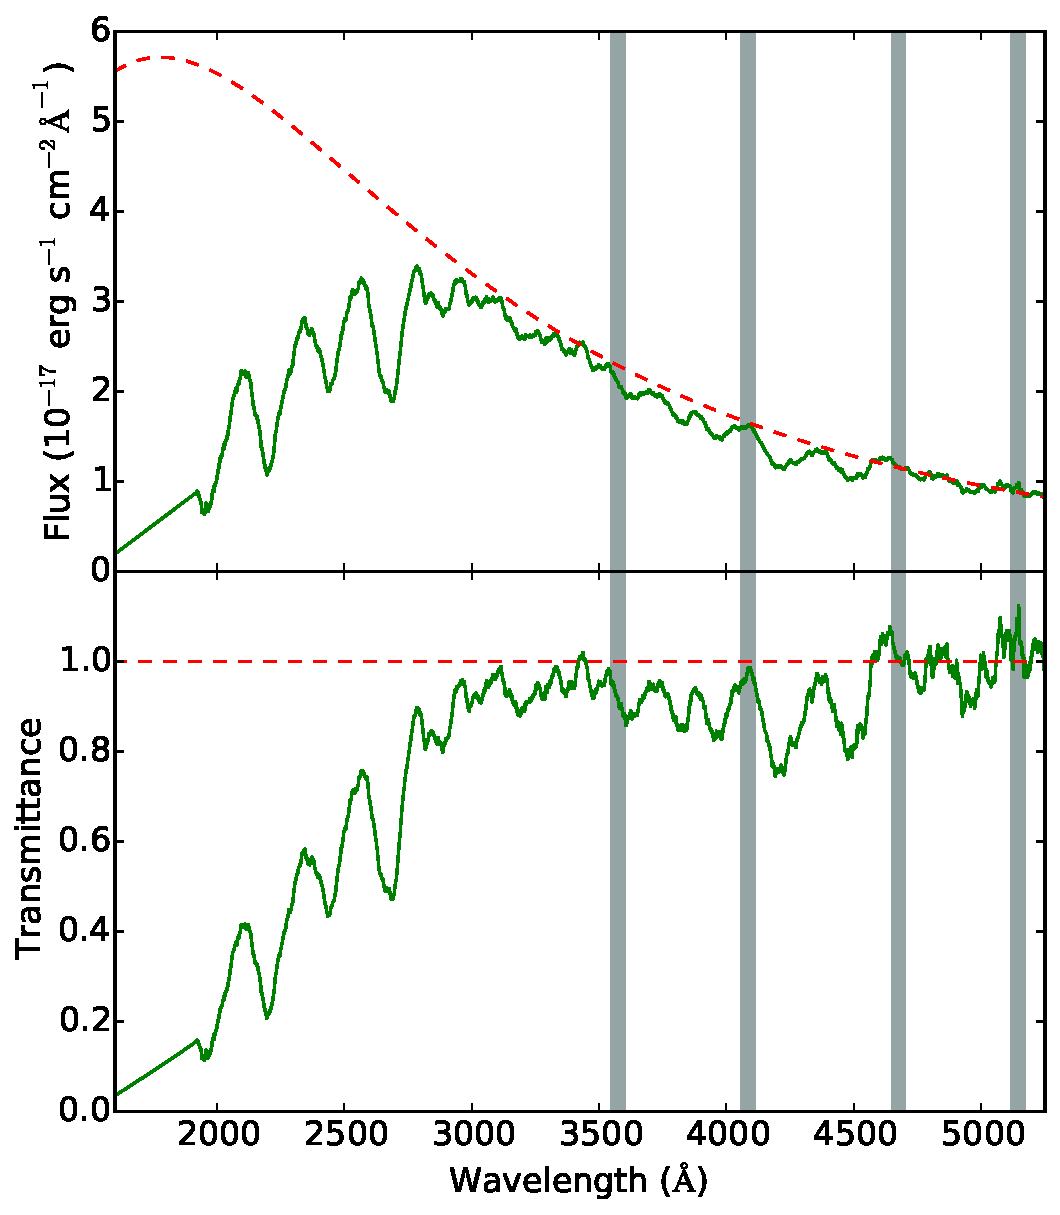
\includegraphics[width=\textwidth]{Figures/Chapter4/specTemplate}
\caption{iPTF13ajg is fitted with the Planck function. The spectrum of iPTF13ajg (green) can shows a good agreement with the blackbody (red) at $\lambda>3000\AA$. At lower wavelengths a strong deviation from the model is observed, highlighting the need for a correction to the model. The ratio between the observed spectrum and the continuum give a measure of the absorption strength as a function of wavelength and can be used in modelling the SLSN SED.}
\label{fig:specTemplate}
\end{figure}

\subsection{Modelling the SED evolution}
The posibility of describing the SEDs of SLSNe as blackbodies greatly simplies the
modelling of its evoution. The model is required to provide only the thermal and radial evolution of the photoshere, therefore removing the need for complex modelling such as radiative transfer or hydrodynamic simulations.

\subsubsection{Fireball model}
Perhaps the simplest approach to modelling the SED evolution is to assume that the SN, with an initial radius R$_{0}$ and initial temperature T$_{0}$ expands at a constant rate while cooling down also at a current rate as seen in \eref{eq:Howell}
\begin{equation}
\label{eq:Howell}
R(t) &= R_0 + \dot{R}t &&\\
T(t) &= T_0 - \dot{T}t &&
\end{equation}
\noindent While such model does not have any physical motivation, \citet{Howell2013} showed that it provides a good, first-order approximation to the light-curves of SLSNe. Due to its simplicity, the model appeared as an attractive prospect for the modelling of SLSN SEDs. However, our testing showed that while it produces a good fit to a SLSN around the maximum light (<+30days) it is not able to capture the slow evolution in the tale of the light curve as seen in \fref{fig:BB_Mag} making in infarable in comparison with the more complex magnetar model.

\begin{figure}
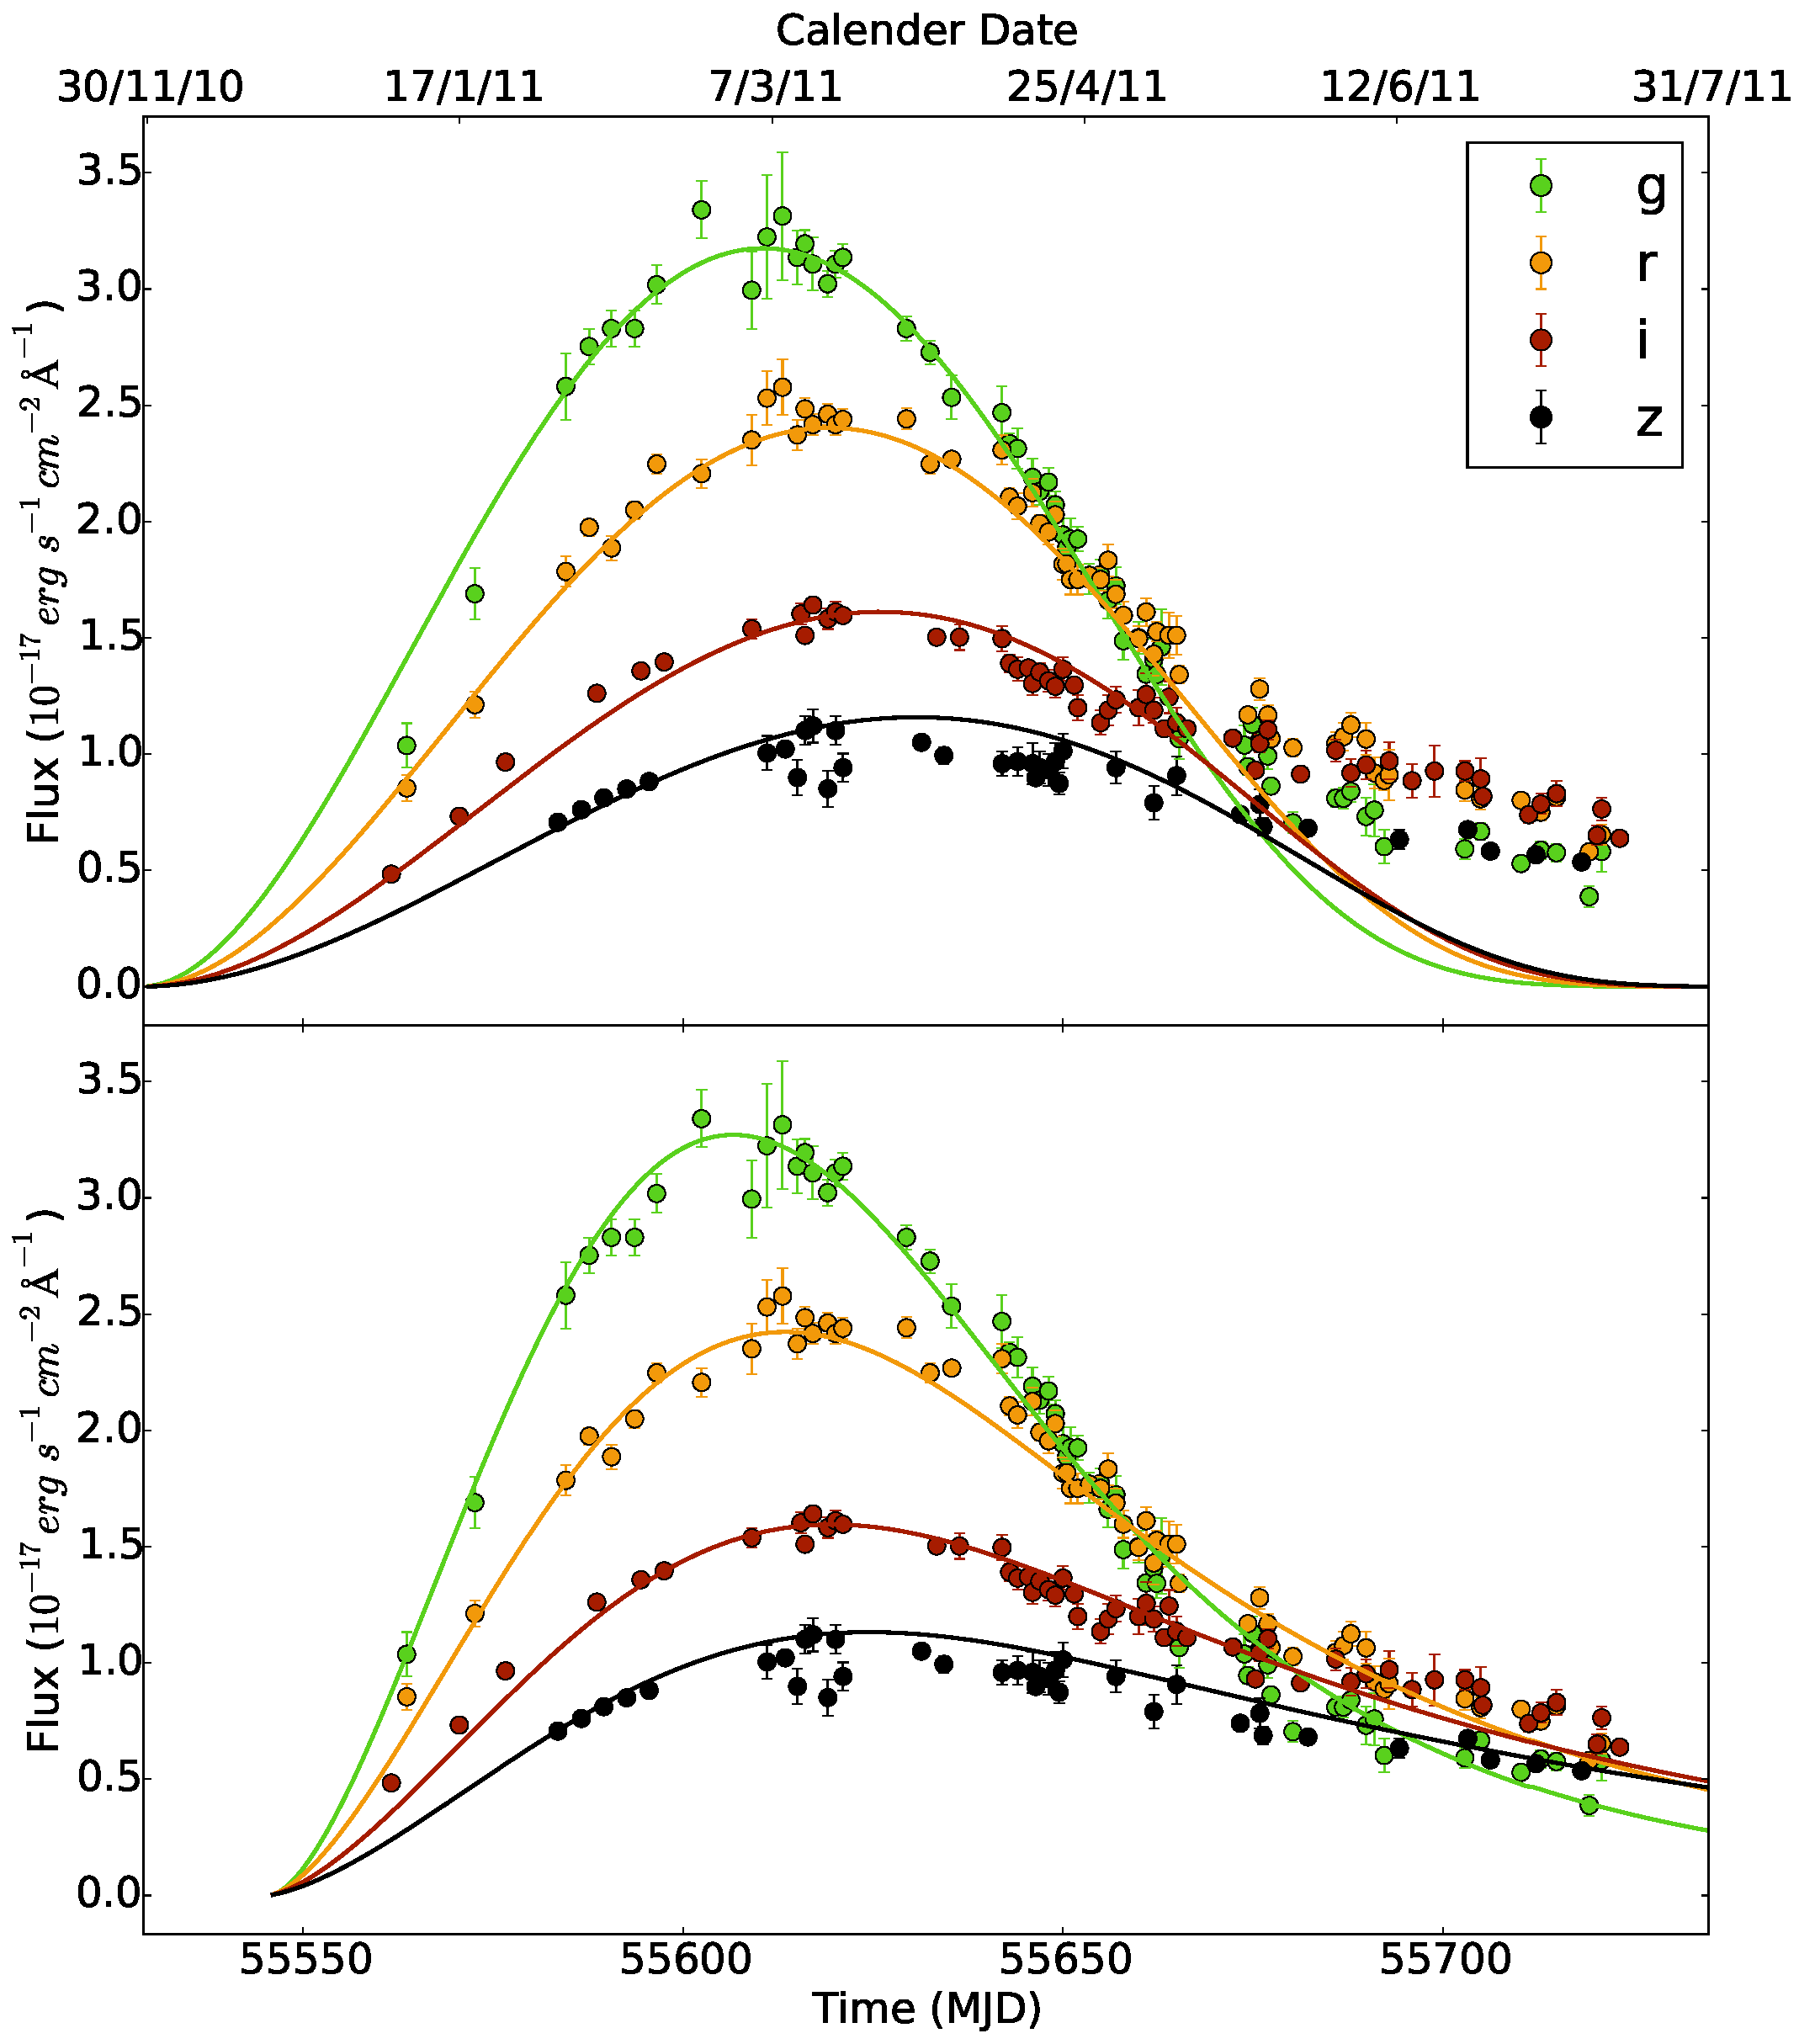
\includegraphics[width=\textwidth]{Figures/Chapter4/BB_Mag_comp}
\caption{The SLSN PS1-11ap $griz$ light curve \citep{2014MNRAS.437..656M} compared to two models describing its photometric evolution. In the upper panel, the model is a simple expanding and cooling blackbody fitted to data around maximum light only, and in the lower panel the model is our `absorbed' magnetar model fitted to the entire light curve. In the case of the magnetar model, the spectrum of SNLS-06D4eu \citep{2013ApJ...779...98H} has been used as an absorption template in the modelling of the SED \sref[see]{sec:KCorrection}). Note that while both models can produce reasonable fits around the peak of the light cuve, the black body model is not able to reproduce the characteristic late-time behaviour of SLSNe. Light curve phases are measured with respect to peak brightness in the rest-frame \textit{u}-band as predicted by our magnetar model fit.}
\label{fig:BB_Mag}
\end{figure}

\subsubsection{Magnetar model}
\label{sec:Magnetar}
To fully capture the evolution of the SED with time we must employ a model for an engine that provides the late time energy deposition needed to explain the photospheric velocity and temperature observed in SLSNe. While still a matter of active debate in literature, in recent years the birth and spin-down of a magnetar model has appeared as the strongest candidate to explain these extremely luminous events \citep{2013ApJ...770..128I,2013Natur.502..346N}. In this model, SLSNe begin as CCSN with a magnetar, a rapidly rotating, highly magnetised neutron star, born at its core. As the magnetar spins down due to the interactions with its environment, it dissipates its energy in the form of high energy radiation that is then captured by the expanding ejecta and thermalised to produce the observed blackbody SED \citep{2010ApJ...717..245K,2010ApJ...719L.204W,2012MNRAS.426L..76D}.

I follow the method from \citet{2013ApJ...770..128I}. In order to model the bolometric luminosity, $L$, of a SLSN as a function of time, $t$, we use equation \ref{Eq:MagnetarLum} based on the Arnett function \citep{1982ApJ...253..785A}.
\begin{equation}
L(t) = 4.9\times 10^{46}\,e^{ -(t / \tau_\mathrm{m})^2 }\delta(t) \int_{0}^{t} \frac{2t'}{\tau_\mathrm{m}^2}\,e^{(t'/\tau_\mathrm{m})^2}\,\frac{B_{14}^{2}\,P_{\mathrm{ms}}^{-4}}{\left(1+t'/\tau_\mathrm{p}\right)^2} dt',
\label{Eq:MagnetarLum}
\end{equation}
\begin{equation}
\label{Eq:SDPeriod}
\tau_{p} = 4.7B_{14}^{-2}P_{ms}^{2}days
\end{equation}
\noindent where $\tau_\mathrm{m}$ is the diffusion timescale, $B_{14}$ is the neutron star magnetic field in units of $10^{14}$\,G, $P_{\mathrm{ms}}$ is the magnetar spin period in ms, $\delta(t)$ is the deposition function or trapping coefficient, and $\tau_\mathrm{p}$ is the magnetar spin-down timescale, is defined in \eref{Eq:SDPeriod}, inferred from $B_{14}$ and $P_{\mathrm{ms}}$. The opacity and total energy parameters have been fixed as $\kappa = 0.1cm^2g^{-1}$ and $E = 10^{51}$erg respectively. It has been shown \citep{2013ApJ...770..128I,2014ApJ...796...87I,2015MNRAS.452.3869N,2015MNRAS.449.1215P} that these parameters only weakly affect the quality of fitting and can therefore be marginalised over.

Physically $\tau_M$ is proportional to the ejecta mass($M_{ej}$) which is sometimes chosen as the fit parameter instead. The two parameters can be converted between each other using equation \ref{Eq:Mej}, where $E$ is the explosion energy and $\kappa$ the opacity of ejecta.
\begin{equation}
\label{Eq:Mej}
M_{ej} = (\frac{\tau_{M}}{10days})^{4/3}(\frac{\kappa}{0.1cm^2g^{-1}})^{-2/3}(\frac{E_k}{10^{51}erg})^{1/3}M_{\odot}
\end{equation}
\noindent The velocity of the ejecta, $v_{core}$ is assumed to be constant and is found using the inferred mass of the ejecta, $M_{ej}$ and its kinetic energy, $E_{mag}$ (\eref{Eq:vcore}), which in turn depends on the explosion energy and the energy released by the spin down of the magnetar (equation \ref{Eq:Emag}). Following the work of \cite{2013ApJ...770..128I,2013Natur.502..346N,2015MNRAS.452.3869N}, constant value of $10^{51}$ erg is used as the explosion energy.
\begin{align}
\label{Eq:Emag}
E_{mag} = 4.9\times10^{46} B^2 P^{-4} \tau_{P}  \text{ erg} \\
E_k = 10^{51} + 0.5 \times E_{mag} \text{ erg}\\
\label{Eq:vcore}
v_{core} =  \sqrt{\frac{10 E_{k}}{3 M_{ej}}} \text{ cm s}^{-1}
\end{align}



Combining this with the total luminosity and the assumption that the object radiates as a blackbody gives us the photospheric temperature. Feed this into the Planck equation gives an approximation for the SED of a SLSN. This method allows for the magnetar model to be fit directly to the multi-band photometry without the need to produce the pseudo-bolometric light curves. We combine this with the absorption templates to produce a model of the SLSN spectral evolution as a function of time.

\paragraph{Trapping coofficient}
The trapping coefficient, $\delta(t)$, is often assumed to be unity
(i.e., implying the full trapping of the high-energy photons radiated
by the magnetar within the supernova ejecta) and time-independent
\citep{2013ApJ...770..128I,2015MNRAS.449.1215P,2015MNRAS.452.3869N}.
Here we use a correction introduced by \cite{2015ApJ...799..107W} with
a time-dependent trapping coefficient of
\begin{equation}
\delta(t) = 1 - \exp\left({-\frac{9\kappa \mathrm{M}_{\mathrm{ej}}^{2}}{40\pi  E_k} t^{-2}} \right),
\label{Eq:Wang}
\end{equation}
where $\mathrm{M}_{\mathrm{ej}}$ is the ejecta mass, $E_k$ is the
explosion energy, and $\kappa$ is the opacity.
$\mathrm{M}_{\mathrm{ej}}$ is proportional to $\tau_\mathrm{m}$, $E_k$
and $\kappa$ \citep{2013ApJ...770..128I}. We fix the explosion energy
to be $E_k = 10^{51}$\,erg and the opacity as $\kappa =
0.1$\,cm$^2$g$^{-1}$ following other studies
\citep[e.g.][]{2013ApJ...770..128I,2014ApJ...796...87I,2015MNRAS.452.3869N,2015MNRAS.449.1215P}.
Using this time-dependent trapping coefficient improves the late-time
fit to the light curve.  For a typical SLSN we calculate $\delta
\simeq 1$ up to 75 days post explosion. However, as the ejecta opacity
to high energy photons decreases with time we find $\delta \simeq 0.8$
at 150 days post explosion, emphasising the importance of this
correction in the late time light curves.

\paragraph{Deriving Radius and Temperature}
We use the equations derived in Appendix D of
\cite{2013ApJ...770..128I} to relate the magnetar model parameters
described above to the photospheric radius and temperature and their
time evolution. The photospheric radius is proportional to the ejecta
velocity, which is also a function of the kinetic energy and
M$_{\mathrm{ej}}$. Thus, using Planck's law the magnetar
model parameters can also be used to generate a simple smooth SED. In
the next section, we discuss how we adjust this SED to physically
resemble the spectra of SLSNe-I.

In its simplest form the model only predicts the total radiated energy of the SN and does not make any predictions about the SED of the object. It is therefore most commonly used with bolometric light curves, synthesised from the photometry. \cite{2013ApJ...770..128I} shows, however, that is is possible to predict the photospheric radius of a SN based on this model.
\begin{align}
r_{core}(t) = v_{core}  t \\
\rho_{core}(t)= \frac{3 M_{ej}}{4  \pi  r_{core}^3(t)}\\
\tau_{core}(t) = \kappa  \rho_{core}(t) v_{core} t
\end{align}
While the radius of the photosphere exceeds that of the core ejecta the radius can be found using equation \ref{Eq:R19}.
\begin{equation}
\label{Eq:R19}
R(t) = r_{core}(t) \left(\frac{\alpha - 1}{\tau_{core}(t)}\right)^\frac{1}{1 - \alpha}
\end{equation}
When the photosphere recedes into the core the radius is instead found by equation \ref{Eq:R20} \citep{2013ApJ...770..128I}.
\begin{equation}
\label{Eq:R20}
R(t) = r_{core}(t) - \frac{1 - \frac{\tau_{core}(t)}{\alpha - 1}}{\kappa \rho_{core}(t)}
\end{equation}

\subsection{SLAP}
text
\subsection{Optimisation}
text
\subsubsection{Least-Squares fitting}
text
\subsubsection{\textsc{MultiNest}}
text
\subsection{pyMagnetar}
text

\section{Searching for Fast Transients}
text
\subsection{Searching for Bumps of SLSNe}
text
\subsection{Searching for Rapidly Evolving Transients}
text

\section{Modeling CCSN}
text
\subsection{CoCo}
text
\subsection{pyCoCo}
text
\subsection{SNIb/c SED UV Extensions}
text
\subsection{SNII with CoCo}
text

\section{Gaussian Processing}
text
\subsection{Theory}
text
\subsection{Choice of Kernels}
text
\subsection{Interpolating Light Curves}
text
